% This is "www2010-sample.tex" copied from "www2005-sample.tex" V1.2 January 26 2004
% This file should be compiled with V1.4 of "www2010-submission.class"
%
% This example file demonstrates the use of the 'www2010-submission.cls'
% V1.4 LaTeX2e document class file. It is for those submitting
% articles to the WWW'04 Conference WHO DO NOT WISH TO 
% STRICTLY ADHERE TO THE SIGS (PUBS-BOARD-ENDORSED) STYLE.
% The 'www2010-submission.cls' file will produce a similar-looking,
% albeit, 'tighter' paper resulting in, invariably, fewer pages.
%
% ----------------------------------------------------------------------------------------------------------------
% This .tex file (and associated .cls V1.4) produces:
%       1) NO Permission Statement
%       2) WWW'04-specific conference (location) information
%       3) The Copyright Line with ACM data
%       4) NO page numbers
%
% ---------------------------------------------------------------------------------------------------------------
% This .tex source is an example which *does* use
% the .bib file (from which the .bbl file % is produced).
% REMEMBER HOWEVER: After having produced the .bbl file,
% and prior to final submission, you *NEED* to 'insert'
% your .bbl file into your source .tex file so as to provide
% ONE 'self-contained' source file.
%
% ================= IF YOU HAVE QUESTIONS =======================
% Questions regarding the SIGS styles, SIGS policies and
% procedures, Conferences etc. should be sent to
% Julie Goetz (goetz@acm.org) or Adrienne Griscti (griscti@acm.org)
%
% Technical questions only to
% Gerald Murray (murray@acm.org)
% ===============================================================
%
% For tracking purposes - this is V1.2 - January 26 2004
\documentclass{www2010-submission}
\usepackage{fancyvrb}

\begin{document}
%
\title{QueryMed: An Intuitive SPARQL Query Builder for Biomedical RDF Data}
%\subtitle{[Extended Abstract]
%\titlenote{A full version of this paper is available as
%\textit{Author's Guide to Preparing ACM SIG Proceedings Using
%\LaTeX$2_\epsilon$\ and BibTeX} at
%\texttt{www.acm.org/eaddress.htm}}}
%
% You need the command \numberofauthors to handle the "boxing"
% and alignment of the authors under the title, and to add
% a section for authors number 4 through n.
%
% Up to the first three authors are aligned under the title;
% use the \alignauthor commands below to handle those names
% and affiliations. Add names, affiliations, addresses for
% additional authors as the argument to \additionalauthors;
% these will be set for you without further effort on your
% part as the last section in the body of your article BEFORE
% References or any Appendices.

\numberofauthors{2}
%
% Put no more than the first THREE authors in the \author command

% NOTE: All authors should be on the first page. For instructions
% for more than 3 authors, see:
% http://www.acm.org/sigs/pubs/proceed/sigfaq.htm#a18

\author{
%
% The command \alignauthor (no curly braces needed) should
% precede each author name, affiliation/snail-mail address and
% e-mail address. Additionally, tag each line of
% affiliation/address with \affaddr, and tag the
%% e-mail address with \email.
\alignauthor Oshani Seneviratne\\
       \affaddr{Massachusetts Institute of Technology}\\
       \affaddr{Cambridge, MA}\\
       \affaddr{USA}\\
       \email{oshani@csail.mit.edu}
\alignauthor Rachel Sealfon\\
       \affaddr{Massachusetts Institute of Technology}\\
       \affaddr{Cambridge, MA}\\
       \affaddr{USA}\\
       \email{rsealfon@csail.mit.edu}
}
\date{15 Feb 2010}

\maketitle
\begin{abstract}
We have developed an open-source SPARQL query builder and result set visualizer for biomedical data, QueryMed, that allows end users to easily construct and run translational medicine queries across multiple data sources. 
\smallskip

QueryMed is flexible enough to allow queries relevant to a wide range of biomedical topics, and runs queries across multiple SPARQL endpoints. It is designed to be accessible to users who are not familiar with the structure of the underlying ontologies used in describing the datasets, or with the SPARQL query language. The system allows users to select the data sources that they wish to use, drawing on their specialized domain knowledge to decide the most appropriate data sources to query.  Users can add additional data sources if they are interested in querying endpoints that are not in the default list. After retrieval of the initial result set, query results can be filtered to improve their relevance.  The system also allows the user to exploit the underlying structure of the RDF data to improve query results. 
\end{abstract}

% A category with only the three required fields
\category{J.3}{Life and Medical Sciences}{Computer Applications}
\category{H.3.3}{Information Search and Retrieval}{Information Systems}

\keywords{Biomedical Ontologies, SPARQL Query Building, Query Federation, Semantic Web, User Interfaces}

\section{Introduction}

The quantity of publicly available data in the biomedical domain has dramatically increased over recent years.   Publicly available biomedical resources include data on drug discovery~\cite{Sharp, Goble}, clinical trials, diseases, disease genes, and phenotypes.  With the linked open data movement, the semantic web community has been very proactive in converting these rich information resources to RDF~\cite{LinkingData}.  In fact, the biomedical domain is among the early successes of the semantic web, due to the rapidity with which the community has made its data available in RDF triple stores \cite{Yip}.  

%The Semantic Web Health Care and Life Sciences Interest Group (HCLSIG) has been formed with the purpose of exploring the applications of the semantic web to the biomedical domain \cite{HCLSIG}.
\smallskip

To allow end users to exploit the abundance of biomedical data that is currently available in RDF, there is a need for easy-to use systems that do not require the end user to have knowledge of the underlying  structure of the data, and that also allow users to run federated queries on multiple SPARQL endpoints.  There is also a  need for efficient hybrid interfaces that allow both browsing and querying data~\cite{Jentzsch}. Many currently available systems are linked data browsers such as the Tabulator~\cite{Tabulator} which permit users to navigate the data in an exploratory manner, but lack support for filtering and querying the data in a user friendly manner.

\smallskip

Answering many medically and biologically relevant questions requires searching, filtering, and combining information from multiple data sources.  For example, a physician may know her patient's personal information, symptoms, current medications, and genotype. She may wish to determine the patient's treatment plan and identify clinical trials for which the patient is eligible.  Although the physician has a single question--``based on the information I have about this patient, what is the best treatment plan and set of clinical trials available?"--there is no single data source that the physician can use to answer this question. The information that the physician needs must be gathered from numerous data sources such as Pubmed, DailyMed, Drugbank, LinkedCT, Diseasome,  and Gene Ontology \cite{Pubmed, DailyMed, Drugbank, LinkedCT, Diseasome, GO}. Her question must be broken up into discrete pieces that can be executed individually at one data source at a time.  

\smallskip

Since the physician must search many data sources in order to find an answer to her single question, she requires a system that can automatically run queries over multiple SPARQL endpoints. Also, the physician may not know SPARQL query syntax, the location of the SPARQL endpoints, or the structure of the relevant ontologies. She is likely to want an intuitive way to query and to display the query results.  Developing intuitive ways to query multiple SPARQL endpoints and to display results is both an important and a challenging problem.  Our system, QueryMed, allows users with no knowledge of the SPARQL query language or the structure of the underlying ontologies to easily run queries across multiple SPARQL endpoints.

\smallskip

This paper is organized as follows:  Section \ref{background} provides background information on the semantic web and its relevance for modeling data in the biomedical domain. Section \ref{system} describes our system. Section \ref{related} discusses related work and illustrates how QueryMed differs from previous systems. Section \ref{future-work} outlines future work. Finally section \ref{conclusion} summarizes the contributions of our system.

\pagebreak

\section{Background}
\label{background}


\begin{figure}
\centering
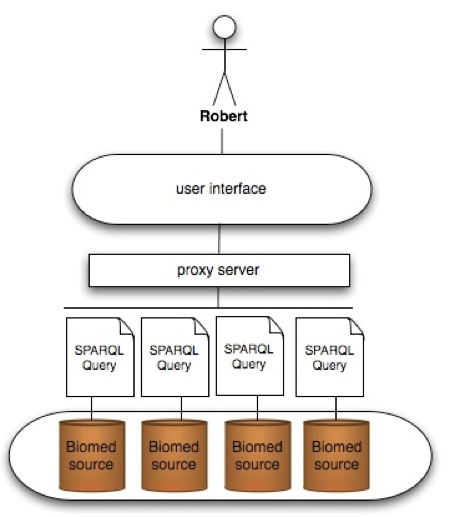
\epsfig{file=images/architecture_overview.jpg}
\caption{QueryMed Architecture Overview}
\label{fig:arch_overview}
\end{figure}


The semantic web can be viewed as a global database system for the information available on the world wide web. Semantic web data is modeled by structured languages such as RDF and OWL, and can be queried using the SPARQL query language. The addition of structure to web data allows inferences to be automatically drawn by intelligent agents integrating data from multiple sources~\cite{Berners-Lee1}.  
%Although most web data are not currently available in semantic web formats, the biomedical knowledge domain has been an early success of the semantic web \cite{Yip}. 

\smallskip

Many major biological and biomedical data resources, including Gene Ontology, DailyMed, LinkedCT, and Diseasome, are currently available as RDF triplestores.   Almost all of these data sources are interlinked. Integrating biomedical data across multiple data sources and automatically extracting specific  knowledge from web resources are crucial tasks for physicians and biologists. These semantic web resources represent valuable repositories of information that can be automatically mined for applications that require biological knowledge.  

\smallskip

Although many valuable resources in the biomedical domain are available in RDF, there are a number of challenges that must be addressed in order to make such resources accessible to physicians, patients, and life scientists.  One challenge is constructing systems that allow end users to run intuitive queries on biomedical data.  Users of biomedical resources are likely to have extensive domain knowledge, but be unfamiliar with query language syntax and with the structure of biomedical ontologies.  Almost all the SPARQL endpoints available today offer generic query interfaces that require users to manually write their queries.  This can be a daunting task  especially for someone who is new to semantic web technologies.  Therefore, it is important to design user-friendly systems that allow users to take advantage of the wealth of structured biomedical knowledge available on the semantic web.  Another central challenge is designing systems that permit users to query multiple data sources simultaneously, since relevant biomedical data are often distributed among many sources \cite{Pasquier}.  

\smallskip


\section{Design \& Implementation}
\label{system}


The QueryMed system allows the user to easily query multiple biomedical data sources.  Queries can be run against a default list of SPARQL endpoints, or against a set of user-selected endpoints.  The end user can easily input additional endpoints in order to utilize resources that are not included in the default list.  The system automatically translates the user input into a SPARQL query for each individual endpoint, executes the query, combines the results, and returns them to the user.  The user can choose to refine the query by iteratively modifying the original query terms, and by filtering the result set.  The advanced query functionality of the QueryMed system allows the user to easily construct complex logical SPARQL queries that take advantage of the underlying structure of the ontologies. The simple user interface of the QueryMed system is designed to be intuitive for users with no knowledge of the SPARQL query language. 

\smallskip

In the following sections we explain the system functionality by first giving an overview of the QueryMed system architecture and the design decisions behind crucial components of the system.

\subsection{QueryMed Overview}

\begin{figure}
\centering
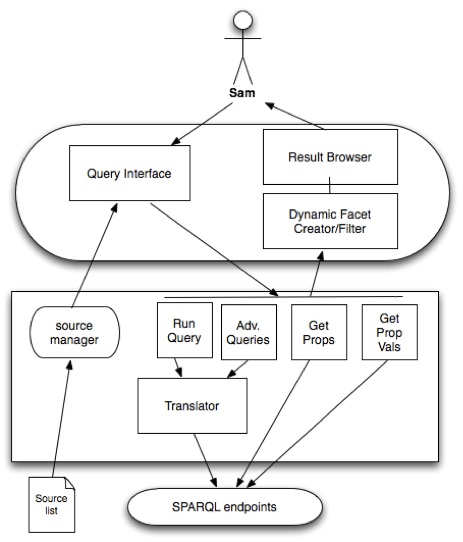
\epsfig{file=images/architecture_detail.jpg}
\caption{QueryMed Architecture Details}
\label{fig:arch_details}
\end{figure}


A general overview of QueryMed architecture is shown in Figure \ref{fig:arch_overview}. The main components of the system are the user interface and the proxy server.   After a user submits a query from the user interface, the query is translated by the proxy server into individual SPARQL queries for each remote endpoint.  The query results are returned from the remote endpoints, combined by the proxy server, and presented to the user.   Figure \ref{fig:arch_details} presents a detailed illustration of the parts of the QueryMed system.  


%The system relies on two external resources: 

%\begin{enumerate}
%\item \textbf{SPARQL endpoints} that expose biomedical data.
%\item \textbf{Sources List} that gives a list of endpoints available to the user. This list is stored on the proxy server, but can be replaced by the user. 
%\end{enumerate}

\subsubsection{User Interface}

The QueryMed user interface is designed to be intuitive for the end user, yet flexible enough to permit a broad range of interesting queries.  The basic query interface allows the user to run simple queries, and is designed for maximal ease of use.  The advanced search capabilities enable the user to easily construct complex logical queries that take advantage of the underlying structure of the biomedical ontologies.  The user interface also allows the user to iteratively refine queries, and displays the query results, which have been retrieved from multiple SPARQL endpoints.  

\smallskip

The main components of the user interface are as follows:

\begin{itemize}

\item \textbf{Basic Query Interface:}  In order to make QueryMed easy to use, but also provide a flexible system that is capable of performing a broad variety of biomedically relevant queries, we provide an uncluttered basic search interface as shown in Figure \ref{fig:initial_ui}. The ``Query All" button performs a keyword-based query over the default set of  data sources. The advanced search option ``Refine Query" allows the user to access the Advanced Query Interface.  

\smallskip

 For example, a physician interested in finding semantic web resources related to coronary artery disease could use ``coronary artery disease"  as a search keyword in the input search box and select the ``Query All" option.   This query searches all default data sources for resources related to coronary artery disease.  The simplicity of the basic query interface allows the physician to rapidly and easily browse semantic web resources of interest. 

\begin{figure}
\centering
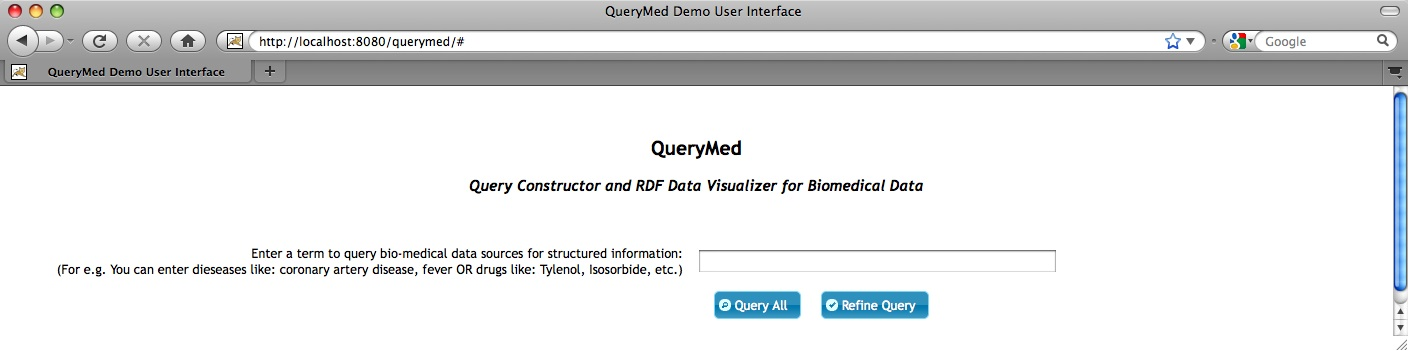
\epsfig{file=images/new_front.jpg,  width=3in}
\caption{Initial Basic Query Interface}
\label{fig:initial_ui}
\end{figure}

\item \textbf{Result Browser:} The user can view her query results organized by source in the Result Browser. The results are presented in a table with pagination.  The user can choose the number of results viewed at a time, search the columns based on some text value and also sort the columns as shown in Figure \ref{fig:results}.  This allows the user to perform additional filtering on the query results to display the most relevant results.  This feature is particularly useful for refining queries that return a large number of results.


\begin{figure}
\centering
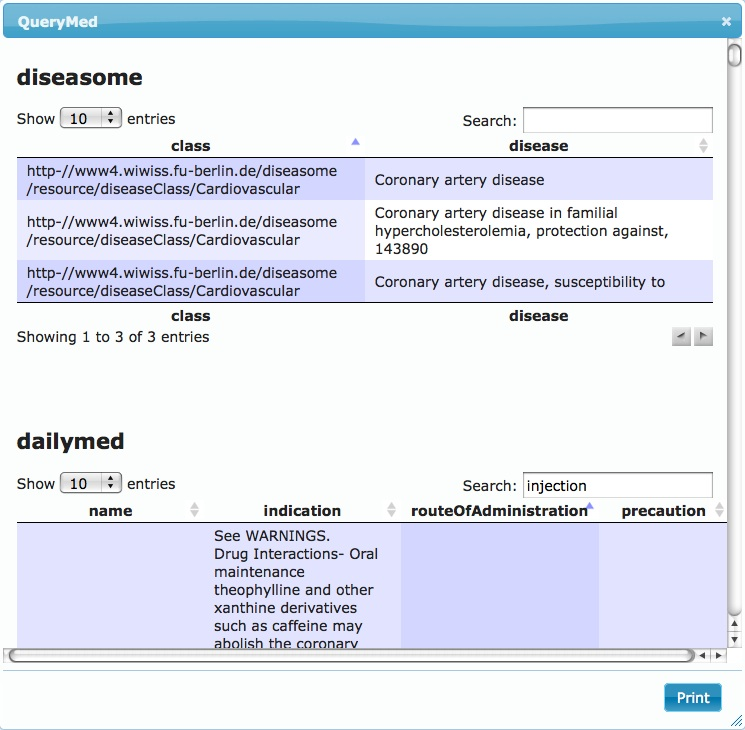
\epsfig{file=images/results.jpg, width=3.5in}
\caption{Sample Result Table}
\label{fig:results}
\end{figure}

\smallskip

For example, after searching for ``coronary artery disease" in the basic query interface, the physician will see displayed in the Result Browser a list of disease names in the Diseasome database and drugs in DailyMed and Drugbank that relate to coronary artery 
disease. She can then filter the results using additional search terms. For example, she knows that 
the route of administration of the drug that she is interested in is injection, so she filters the drug query results on the route of administration field using the query term ``injection."   The additional filtering capabilities of the Result Browser allow her  either to browse a large number of query results, or refine her search to view only the most relevant results.

\item \textbf{Advanced Query Interface:} The Advanced Query Interface allows the user to add new data sources, and to construct a complex SPARQL query that takes advantage of the structure of the underlying biomedical ontologies.  Thus, the end user can construct a targeted query without previous knowledge of the SPARQL language or the structure of the relevant ontologies.

When the ``Refine Query" in the Basic Query Interface is invoked, the user is provided with the default list of data sources as shown in Figure \ref{fig:select}.  The user may select from this list relevant data sources that they wish to query.  The user can also dynamically add additional data sources as shown in Figure \ref{fig:add_source}, allowing her to query endpoints of interest that are not included in the default list.

A physician who is interested in using the QueryMed system to find relevant clinical trials for 
her patient can use the Advanced Query Interface to add additional relevant datasources.  For example, she might want to use the clinical trial database LinkedCT, which is 
not in the default set of endpoints.  So, she selects the �Refine 
Query� option to select the endpoints to search, and then the �Add� option 
to include an additional endpoint. After entering the name 
and URL of the LinkedCT endpoint, she can able to search 
for clinical trials for which her patient may be eligible. 

\begin{figure}
\centering
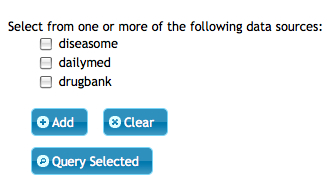
\epsfig{file=images/select.jpg,  width=2.5in}
\caption{The user has the option of selecting specific trusted or relevant data sources, or of adding additional data sources to query.}
\label{fig:select}
\end{figure}


\begin{figure}
\centering
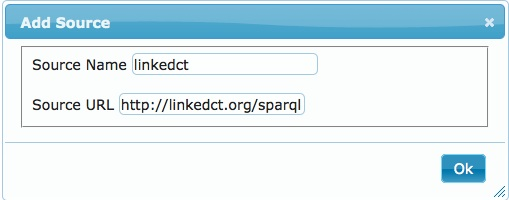
\epsfig{file=images/add_source.jpg,  width=3in}
\caption{The user can dynamically add additional SPARQL endpoints.}
\label{fig:add_source}
\end{figure}

When a data source is selected, the properties list is automatically populated with all distinct properties available at the selected endpoint. The user can specify values for relevant properties to restrict the search space.
%The properties list is generated by running a SPARQL query of the form given in Figure \ref{fig:SPARQL_props} at the specified data source. 

\smallskip

Once the properties are returned, they will be displayed in the user interface as shown in Figure \ref{fig:add_props}. Clicking an individual property link displays a description of the property. This allows the user to understand the keywords that will be most useful to search on each specific property. 

\smallskip

The user can choose to perform exact queries, or filter results on specific keywords. If the user does not know the specific value for a property, she can instead specify a keywords using the �FILTER� option. She also can choose logical operators to connect the various parts of her query. When �AND� is used it will be appended as a basic triple pattern to the SPARQL query, i.e. as a conjunction. When �OR� is used, the specified graph pattern is made to disjunct with the rest of the query with the SPARQL UNION operator. If no logical operator is specified, �AND� will be used by default.  The advanced query feature is capable of dynamically constructing complex SPARQL queries, such as the query shown in Figure \ref{fig:SPARQL_adv}.

\smallskip

For example, the physician might want to further refine her search for cardiovascular diseases. She 
uses the advanced search option to construct a boolean query 
that takes advantage of the underlying structure of the RDF 
data in the database. She searches Diseasome for 
diseases whose class is ``Cardiovascular" or for which the associated gene is �ABCA1.� Using the QueryMed advanced 
search interface, the complex SPARQL query corresponding 
to her question is automatically constructed (Figure \ref{fig:SPARQL_adv}), and she can 
view the query results conveniently displayed in the Results Browser.


\begin{figure}
\begin{Verbatim}[frame=single]
SELECT distinct ?disease WHERE { 
{?x <http://www.w3.org/2000/01/rdf-schema#label> 
?disease 
FILTER regex(?disease, 
"coronary artery disease", "i"). 
?x <http://www4.wiwiss.fu-berlin.de/diseasome/
resource/diseasome/class> 
<http://www4.wiwiss.fu-berlin.de/diseasome/
resource/diseaseClass/Cardiovascular>} 
UNION { ?x <http://www4.wiwiss.fu-berlin.de/
diseasome/resource/diseasome/associatedGene>
 <http://www4.wiwiss.fu-berlin.de/diseasome/
 resource/genes/ABCA1>.}
}
\end{Verbatim}
\caption{A complex SPARQL query that was dynamically constructed using the advanced query feature of the QueryMed system.}
\label{fig:SPARQL_adv}
\end{figure}

\begin{figure*}
\centering
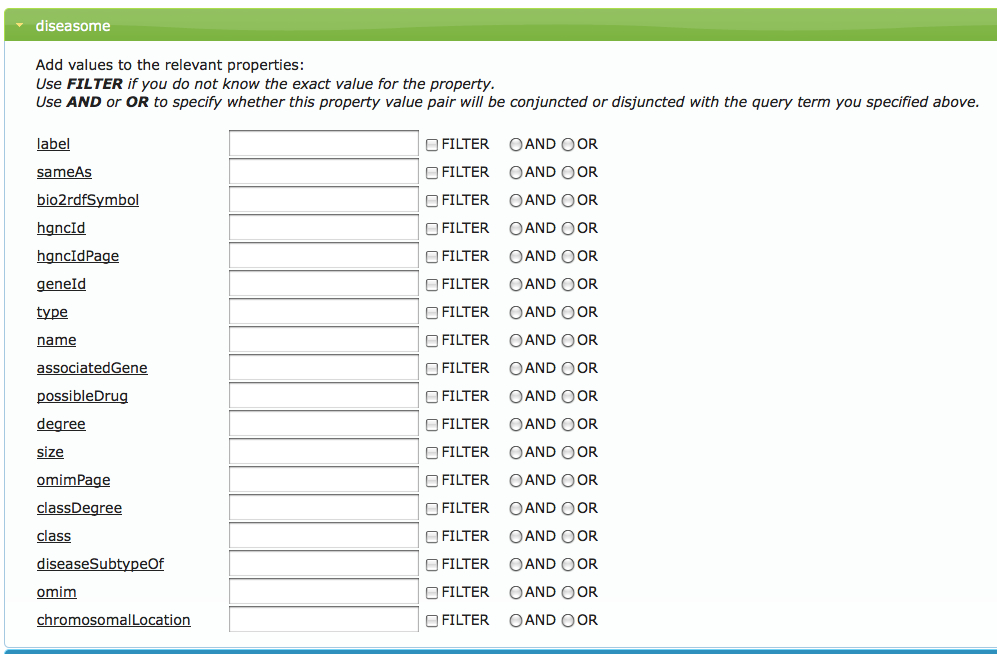
\epsfig{file=images/add_props.jpg, width=6in}
\caption{The advanced search feature allows the user to perform exact or pattern-matching queries connected by user-specified logical operators over specific properties in given resources, taking advantage of the structure in the RDF data.}
\label{fig:add_props}
\end{figure*}

\item \textbf{Dynamic Facet Creator/Filter:} The Dynamic Facet Creator/Filter allows the user to select a  set of  data sources, load the properties available at these sources, and dynamically construct a complex SPARQL query connected by logical operators to take advantage of the structure of the data at each endpoint (Figure  \ref{fig:facet_creator}). The interface allows displaying of many property lists from different sources simultaneously (grouped by source). Therefore, only information relevant to the endpoint the user is currently examining will be visible at any given time.

\begin{figure}[h]
\centering
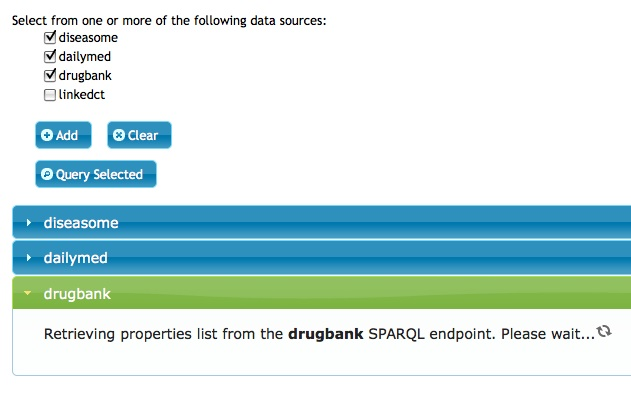
\epsfig{file=images/facet_creator.jpg, width=3in}
\caption{Dynamic Facet Creator and Filter}
\label{fig:facet_creator}
\end{figure}

\end{itemize}

\subsubsection{Proxy Server}

The proxy server acts as an intermediary between the user interface and the remote SPARQL endpoints.  Its functionality is twofold: 

\begin{enumerate}
\item Execute the SPARQL queries at the relevant remote SPARQL endpoints and consolidate the results to be presented in the user interface.
\item Cache the results of the current query so that refinements of the query will have reduced network and query execution latency.
\end{enumerate}

The specific components in the Proxy Server are as follows.

\begin{itemize}



\item \textbf{Source Manager:} The Source Manager reads the source list and populates the default query list on the user interface. It also manages the default endpoints, the currently selected endpoints, and the endpoints that have been dynamically added.

\item \textbf{Translator:} The Translator is responsible for translating the user query into valid SPARQL syntax.  The Translator obtains the parameters to construct the query from the input the user specifies in the Query Interface, and dynamically constructs a SPARQL query based on the user input. The Translator relies on two services:

\begin{enumerate}

\item \textbf{Run Query:} The purpose of this service is to execute SPARQL queries generated by the Translator, and return  the query results as a JSON object.



%\begin{figure}
%\begin{Verbatim}[frame=single]
%{
%   "bindings":
%  [
%        {"source" : "source_label",
%         "uri" : "http://source.com/sparql.",
 %    	"vars" : ["variable1","variable2"],
  %   	"count":2,
   %  	"results" : 
   %  	 [
  %   	    {"variable1": "Value 1",
%	      "variable1": "Value 2"},
 %    	    {"variable1": "Another Value 1",
  %             "variable1": "Another Value 2"},
 %  	    ...	  		
  %   	 ]
  %   	}
  %   	,
%	{ //Another Source and Result Description
%	...
%	},
%	...
 %    ]
% }
%\end{Verbatim}
%\caption{Structure of the JSON ``result" object}
%\label{fig:JSON_runquery}
%\end{figure}

\item \textbf{Advanced Queries:} This service takes as input list of sources, properties, query terms, and logical operators, which are passed to the proxy server as a JSON object.

%\begin{figure}
%\begin{Verbatim}[frame=single]
%{
% "http://some-source/sparql": 
%  {
%     "property1": {"value1":  "logical operator"},
%     "property2": {"value 2": "logical operator"},
%     "property2": {"value 3": "logical operator"},
%     ...
%  }
%}
%   //Other sources ...

%\end{Verbatim}
%\caption{Structure of the JSON ``query" object}
%\caption{JSON constructed to send the structure of a SPARQL query for an advanced query with logical operators}
%\label{fig:JSON_advquery}
%\end{figure}


\end{enumerate}

% The user has to specify the data source(s) to query, and can give specific values for one or many of the properties available for the data available to restrict the query space. 

%\item \textbf{Additional Services:} In order to make the user interface more user friendly, the following two services perform some ``behind the scenes" work.

%\begin{enumerate}
%\item \textbf{Get Properties:} This service takes as input an individual source, and returns an array of all properties for that source.
%\item \textbf{Get Property Values:} This service takes as input an individual source and a specific property.  It returns a list of the possible values that this property can take.
%\end{enumerate}

\end{itemize}

\subsection{Design Decisions}

\subsubsection{Source list}

Because the set of default endpoints is stored on the proxy server, the set of resources available by default to the user can easily be updated.  Since useful biomedical resources are rapidly being developed and made available as RDF triple stores, the ease of updating the resource list ensures that the system can easily be brought up to date. In fact, the QueryMed system could easily be adapted to perform queries outside the biomedical domain by modifying the list of input data sources.

\subsubsection{Proxy Server}

While an entirely client side application is possible, we chose to have a proxy server perform the SPARQL query execution and caching. This design is advantageous for several reasons:

\begin{enumerate}

\item Efficient cache management: The result set from running an unrestricted query can include millions of results. It may be infeasible to keep unfiltered query results in browser memory. A typical memory footprint for a browser (for e.g. Firefox) is usually between 20MB and 100MB. A poorly constructed query can result in gigabytes worth of triples returned, causing the browser to crash. The proxy server can cache results from initial query execution, so that only a filtered result set is subsequently returned to the client.

\item The proxy server, and not the Javascript client, executes SPARQL queries at the remote endpoints. This avoids cross domain XML-HTTP-Request errors in accessing web servers at various domains that are used to host the remote biomedical SPARQL endpoints.

\end{enumerate}


\begin{figure}
\begin{Verbatim}[frame=single]
SELECT ?projection_1 ?projection_2 ... 
	?projection_n
WHERE {?x source:property ? projection 
	FILTER regex(? projection, '" + 
	input +"', 'i)
}
... //Other property filers are to follow
\end{Verbatim}
\caption{The structure of the SPARQL query constructed when the user selects ``Query All".}
\label{fig:min_query}
\end{figure}


\subsubsection{Data Structures}

The parameters required for constructing the SPARQL queries are sent from the user interface to the proxy server. In the general ``Query All" case, the system will take the user-specified query term as text-box input, filter on all the triples available at the SPARQL endpoint to select only those that contain the keyword, and display the results. The generated SPARQL query will be of the form illustrated in Figure \ref{fig:min_query}. The word ``input" in the figure represents the keyword specified by the user.

\smallskip

When the results are returned, each result set is structured as a JSON object. This object identifies the endpoint where the query was executed, the URI of the endpoint, the query variables,  how many results are returned and the result set.

\smallskip

When the user runs an advanced query, the proxy server takes as input the data sources to be queried, the properties to be queried, the values for each of the selected properties, and the relationship between the property-value pairs and the original user-specified query term. This information is also passed to the proxy server as a JSON object.


\subsubsection{Query Interface}

The basic query interface is designed to be as simple as possible, so that users who have little previous experience running queries on SPARQL endpoints can easily and rapidly find query results.  The advanced query functionality of our system allows users the flexibility to intuitively construct complex SPARQL queries. 
\subsubsection{Implementation}

QueryMed is implemented in Java in the backend and JavaScript, HTML and CSS in the frontend.  In the backend, the Jena library \cite{McBride} is used to run the SPARQL queries and 4-store~\cite{4store} is used as a triple store to provide caching support.  The JQuery library \cite{Resig} was used to develop an attractive user interface.   

%\subsection{A Sample Use Case}

%A physician is interested in finding semantic web resources related to coronary artery disease.  She first tries a basic search over all default resources, by entering ``coronary artery disease" in the input search box.   She then sees a list of disease names in the Diseasome database and drugs in DailyMed and Drugbank that relate to coronary artery disease displayed in a table.  She can then filter the results using additional search terms.  For example, she knows that the route of administration of the drug that she is looking for is injection, so she filters the drug query results on the route of administration field using the query term ``injection."  She then prints the table of results.

%She is now interested in finding relevant clinical trials for her patient.  However, the clinical trial database LinkedCt is not in the default set of endpoints, so she selects the ``Refine Query" option to choose additional endpoints to search.  She sees a list of default endpoints, and selects the ``Add" option to include an additional endpoint.  After entering the name and URL of the LinkedCT endpoint, she is able to search for clinical trials for which her patient may be eligible.  

%She is also interested in further refining her search.  She uses the advanced search option to construct a boolean query that takes advantage of the underlying structure of the RDF data in the database.  She searches diseasome for a list of diseases whose class is ``Cardiovascular" or for which the associated gene is ``ABCA1."  Using the QueryMed advanced search interface, the complex SPARQL query corresponding to her question is automatically constructed, and she can view the query results conveniently displayed in a table.


\subsection{Performance}

\begin{table*}
\begin{center}
%\begin{tabular}{|l|l|l|l|l|l|l|l|l|l|l|}
\begin{tabular}{| l | p{1.2cm}| p{1.2cm} | p{1.2cm} | p{1.2cm} | p{1.2cm} | p{1.2cm} | p{1.2cm} | p{1.2cm} |}
\hline
& \multicolumn{2}{c}{\textbf{Dieseasome} } \vline & \multicolumn{2}{c}{\textbf{Dailymed}} \vline & \multicolumn{2}{c}{\textbf{Drugbank}} \vline & \multicolumn{2}{c}{\textbf{Sider}} \vline \\
\hline
& \textbf{Without Caching} & \textbf{With Caching} & \textbf{Without Caching} & \textbf{With Caching} & \textbf{Without Caching} & \textbf{With Caching} & \textbf{Without Caching} & \textbf{With Caching} \\
\hline
\textbf{1st Trial}   & 3.45 s &  134 ms & 1.77 s &   384 ms & 9.51 s & 60 ms & 14.64 s & 23 ms \\
\hline
\textbf{2nd Trial}  & 1.61 s & 31 ms & 1.57 s &  32 ms  & 9.34 s & 31 ms & 2.94 s & 7 ms \\
\hline
\textbf{3rd Trial}  & 1.71 s &  7 ms & 1.66 s &   11 ms & 9.06 s & 23 ms & 2.86 s & 6 ms\\
\hline
\end{tabular}
\caption{Running times to retrieve all the properties from selected endpoints}
\label{timing}
\end{center}
\end{table*}


We observed that the slowest step in running queries using the QueryMed system is populating the property values for each selected endpoint.  We compared the times required to load properties from several endpoints, by running the query illustrated in Figure \ref{fig:SPARQL_props}.  Timing data are shown in Table \ref{timing}.

\smallskip

For all selected endpoints, without local data (i.e. no cache on the proxy server), the property values took longer to load.  The difference in running time between \emph{with local data} and \emph{without local data} is approximately three orders of magnitude.  The network latency and the slow performance of the remote SPARQL endpoints as compared to the local data cache explains  the increase in running time for the queries in the two cases.  We also noted that the running time of the subsequent iterations of the same query is significantly less than the initial query, probably due to browser caching. When comparing query execution times across the data sources, we see that the Drugbank takes the longest, probably due to the greater size of the Drugbank dataset as compared to the other three datasets.\footnote{As of February 15\textsuperscript{th} 2010, Diseasome contains 91,182 triples, DailyMed contains 164,276 triples, Sider contains 192,515 triples, and DrugBank contains 765,936 triples) \cite{Diseasome, DailyMed, Sider, Drugbank}}

\smallskip

Based on the dramatic improvement in running time obtained using caching, the slowest step in executing queries with our system is retrieving triples from slow remote SPARQL endpoints.  By managing our own cache to contain the data most likely to be needed on the proxy server, we were able to decrease running time considerably.

\smallskip

\begin{figure}
\begin{Verbatim}[frame=single]
SELECT DISTINCT ?property
WHERE { [] ?property [] }
ORDER BY ?property
\end{Verbatim}
\caption{SPARQL query to retrieve all properties. This was used to measure the performance of implementing a local cache.}
\label{fig:SPARQL_props}
\end{figure}


\begin{figure}
\centering
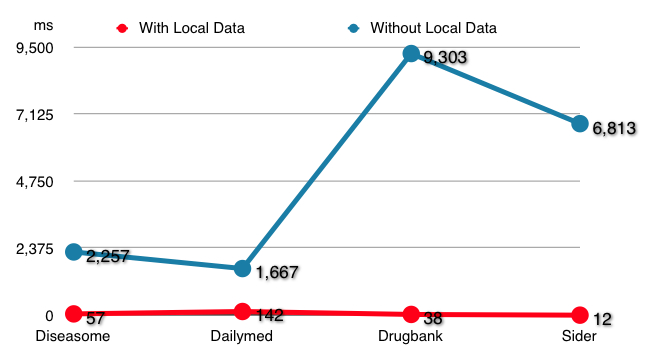
\epsfig{file=images/chart.jpg, width=3in}
\caption{Comparison of query execution times \emph{(ms)} with and without local data caching. The data points represent the average of three trials.}
\label{fig:chart}
\end{figure}

\pagebreak

\subsection{QueryMed Resources}

The source code for the Querymed system is available at the QueryMed Google Code project: \\
http://code.google.com/p/querymed

\smallskip

A video illustrating a sample use case can be found at: \\
http://dig.csail.mit.edu/2010/Papers/www-ws-colab-science/\\
videos


\section{Related Work}
\label{related}

\begin{table*}
\begin{center}
\begin{tabular}{| p{1.8cm} | p{2cm} | p{1.8cm} | p{1.8cm}| p{1.8cm}| p{1.8cm}| p{1.8cm}| p{1.8cm} |}
\hline
 & \textbf{Hybrid Interface (Combines Querying \& Browsing)} & \textbf{Provides Local Caching} & \textbf{Queries Multiple Sources} & \textbf{Dynamic Addition of Sources} & \textbf{Allows Keyword Queries} & \textbf{Open Source} & \textbf{GUI} \\
\hline
\textbf{QueryMed}  & Yes & Yes & Yes & Yes & Yes & Yes & Yes  \\
\hline
\textbf{SMART}  & No & Yes & Yes & No & No & Yes & Yes  \\
\hline
\textbf{DARQ}  & No &  No & Yes & Yes & No & Yes & No  \\
\hline
\textbf{GoWeb}   & Yes & No  & Yes & No & Yes & No & Yes  \\
\hline
\textbf{BioGateway}   & Yes & Yes & Yes & No & No & Yes & Yes  \\
\hline
\textbf{Twinkle}   & No & No & Yes & No & No & Yes & Yes  \\
\hline
\end{tabular}
\caption{Comparison of selected features of the QueryMed system with other related systems.}
\label{comparison}
\end{center}
\end{table*}

A number of existing tools aim to provide a user-friendly interface for browsing biomedical semantic web data, or to allow users to perform federated queries.  Several of these are described below.

\smallskip

The SMART query tool is a web-based application designed to allow biologists to run SPARQL queries over multiple endpoints.  Queries to the SMART system are written in the natural-language like Manchester OWL syntax \cite{Battista}.  Major differences between the QueryMed system and SMART include the ability to construct queries intuitively by specifying keywords for user selected properties, to iteratively refine query results, and to dynamically add additional endpoints in the QueryMed system. 

\smallskip

GoWeb and BioGateway are two additional systems designed for answering queries on biomedical data  \cite{Dietze, Antezana}.  GoWeb allows users to perform a hybrid search, running keyword-based queries and then filtering based on ontological concepts. However, while GoWeb functions as a search engine that incorporates ontological background knowledge to improve search results, QueryMed is a query translation system that utilizes user input in constructing SPARQL queries.  BioGateway provides a web interface to query a provided SPARQL endpoint that includes graphs from several biomedical resources.  However, BioGateway does not allow the user to run queries over multiple endpoints or to dynamically add endpoints.

\smallskip

Twinkle offers a stand-alone graphical user interface to load and edit SPARQL queries that can be used to query online SPARQL endpoints \cite{Dodds}. Our system differs from the Twinkle system in several aspects. First of all, in Twinkle, the user is expected to know what is already available at the SPARQL endpoints to write the query. But in QueryMed, the user can provide input in the form of keywords, and has the option to restrict the query if she wishes to run a more precise query. Second, although Twinkle was designed to be a more general purpose system, it only supports a small number of specific SPARQL endpoints, while QueryMed allows the user to dynamically add SPARQL endpoints.

\smallskip

Most SPARQL query engines are designed to run queries against individual endpoints. But it is often useful to draw on multiple web resources in answering a query. The DARQ  system \cite{Quilitz} is designed to allow the user to run integrated queries against multiple SPARQL endpoints. But it does not offer a graphical user interface to facilitate use by biomedical domain experts who are not familiar with SPARQL query syntax.

\smallskip

Table \ref{comparison} compares selected features of the QueryMed system with other related systems. 

\section{Future Work}
\label{future-work}

Our system currently allows only a restricted set of SPARQL queries. Supporting additional types of queries and including query optimization functionality could increase both the flexibility and the speed of the QueryMed system. By drawing on the expressivity of the SPARQL language and the information contained in the ontologies used to represent the data, it would be possible to extend our system into an intelligent reasoning system on biomedical data which allows physicians to enter sophisticated, complex queries and find relevant biomedical results.

\smallskip

Another approach that could reduce running time still further, especially for users with a slow network connection, would be to create a complementary standalone application that gives the user the option at startup time of loading all the required RDF data. Since data is stored locally after the initial startup, using the system in subsequent queries will be rapid after an initial loading phase.  This approach might be too memory-intensive if the user wishes to run queries over many large triple stores, but might work best in a situation where there is a small or moderate amount of data in the repositories of interest to the user. 

\smallskip


We also believe that it would be useful to allow exploration of the relationships among multiple data sources containing similar resources.  One challenge in integrating biomedical data across multiple sources is that individual data items (i.e, a specific protein or a specific drug) may be represented by distinct URIs at different endpoints. The diversity of representations of identical data items across different biomedical data sources makes it difficult to automatically combine these items.  However, there is some cross-referencing between the biomedical data sources that we included by default in our system.  For example, DailyMed drugs sometimes refer to diseases in the Diseasome data source by their URI.  It might be useful to provide a representation of the relationships among search results from different sources with the query results. Additionally, the system could automatically detect similar data items even if they are identified by different URIs, and group similar items from distinct data sources together in the query results by natural language processing.  Another useful feature might be to allow the user to view the relationships among URIs (as in the relfinder system \cite{Heim} , which displays possible paths through the RDF graph between distinct resources).

\smallskip

We are also working on an autocompletion feature to automatically retrieve the values for any given property. This feature will allow the user to automatically see all valid choices for each property, and will make the system easier to use and reduce empty query result sets.

\smallskip

Since a major goal of QueryMed is ease of use by physicians, life scientists, and patients, we also plan to perform a user study to understand how effectively  users without knowledge of SPARQL can interact with our system.  We plan to use data from this study to further refine our system to improve its usability.

\section{Conclusion}
\label{conclusion}

The QueryMed system  allows endpoints to be dynamically added by the user, and provides a hybrid interface that enables the user to both query and browse data. QueryMed also allows the user both to perform keyword queries and to construct more advanced queries taking advantage of the structure of the data. Furthermore, the Javascript-based user interface of the QueryMed system, implemented using the JQuery UI library, is particularly attractive, easy to interact with, and capable of handling a variety of user input events.  We believe that developing systems such as such as QueryMed, which makes SPARQL endpoints  easily accessible to end users, will entice more people to expose their data as linked open data sources.

\smallskip

The main contributions of our system are: dynamic construction of complex SPARQL queries based on intuitive user input; dynamic addition of user-specified endpoints; and the ability to run queries over multiple endpoints. Because our system is flexible and easy to use, we believe it will be of use to the biomedical community.  

\smallskip


%\section{Acknowledgments}

\bibliographystyle{abbrv}
\bibliography{references}  

\end{document}
